\chapter{Progetto}
\label{sec:arch}

Alla luce delle considerazioni esposte nel capitolo precedente, tenendo conto che riscrivere l'intero microservizio in Rust con Vulkan non sia un lavoro banale (e comunque non ci sarebbero miglioramenti tangibili in termini di prestazioni), si è scelto di adottare un approccio ibrido e, quindi, di mantenere i kernel in \gls{CUDA} e usare Rust per la parte web del microservizio. Questo permette di mantenere le prestazioni e il \textit{know-how} di \gls{CUDA} e di poter trarre benefici l'ecosistema e la \textit{development experience} di Rust. Inoltre, l'uso di Rust per la parte web permette di avere un sistema più sicuro rispetto al C++, e soprattutto più portabile e facilmente mantenibile, grazie al suo sistema di gestione delle dipendenze e alla sua capacità di compilare codice per diverse architetture.

\begin{figure}[ht]
    \centering
    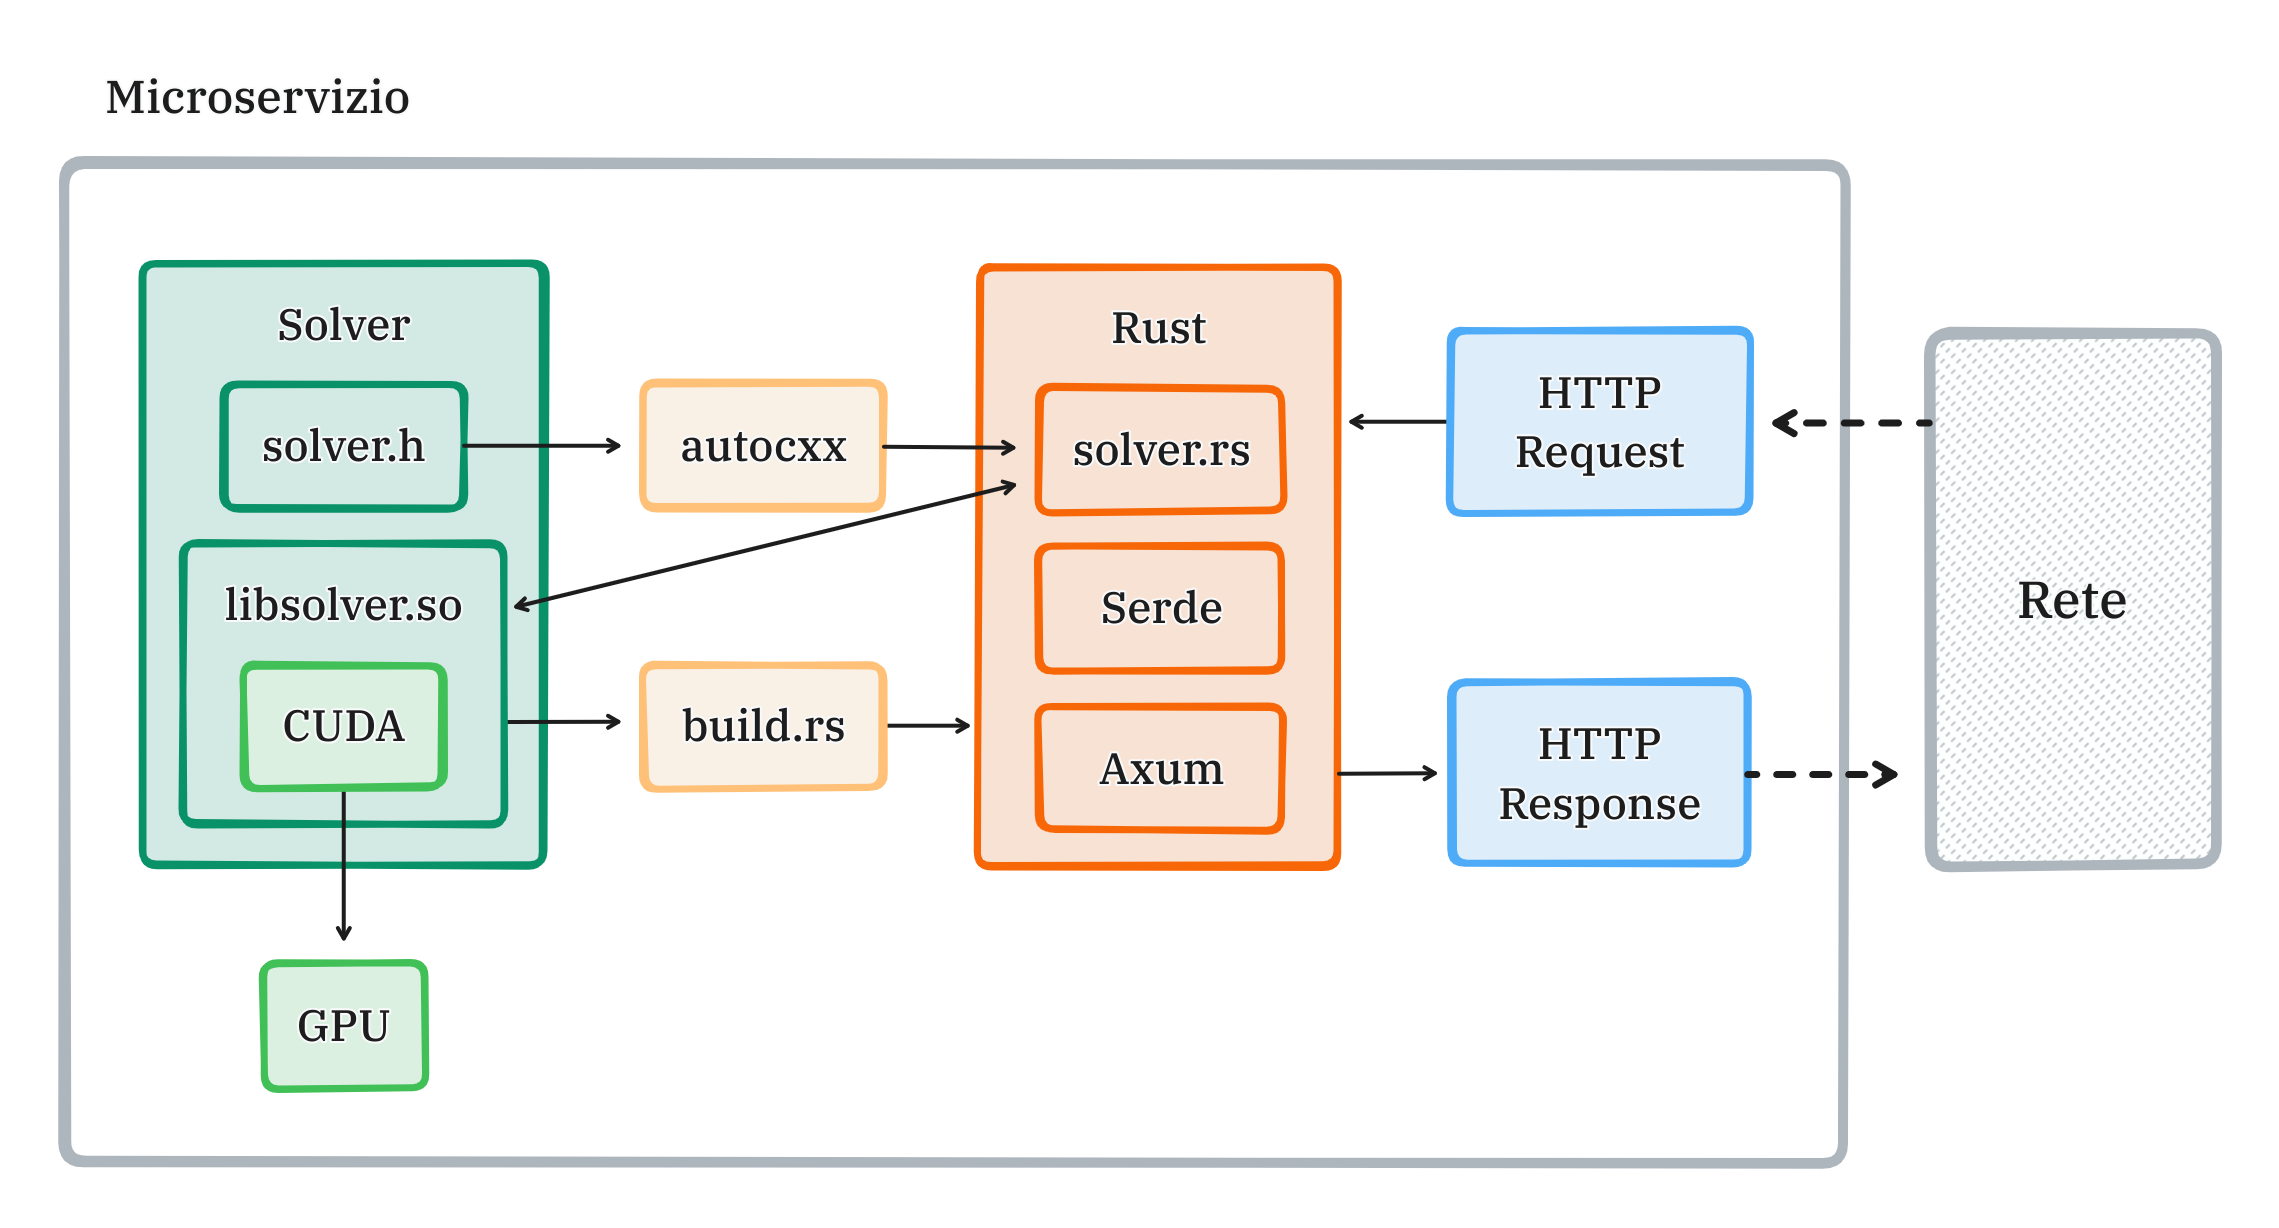
\includegraphics[width=.94\linewidth]{images/chapter6/micro_arch.png}
    \caption{Architettura del microservizio}
    \label{fig:micro_arch}
\end{figure}

\section{Struttura del microservizio}

Mentre in fig. \ref{fig:micro_arch} è mostrato lo schema logico del microservizio, che illustra tutti i componenti essenziali, in \ref{lis:tree} è presente la struttura delle cartelle del progetto. Il progetto è strutturato in modo da separare il codice Rust dalla libreria dinamica in \gls{CUDA}, in modo da poter gestire facilmente le dipendenze e le configurazioni di compilazione.

\vspace{5mm}
\begin{lstlisting}[language=bash, caption=Directory del progetto, label=lis:tree]
$ tree .
.
|-- build.rs
|-- Cargo.toml
|-- lib
|   |-- libsolver.so
|   \-- solver.h
\-- src
    |-- main.rs
    |-- solver.rs
    \-- models.rs
\end{lstlisting}
\vspace{5mm}

Il file \textit{Cargo.toml} contiene le dipendenze del progetto, mentre nel file \textit{build.rs} sono presenti le istruzioni necessarie per il linking della libreria dinamica \verb|libsolver.so| di \gls{CUDA} specificando l'header da cui recuperare la \textit{signature} delle funzioni con \textit{autocxx}, come mostrato in \ref{lis:build_rs}. La cartella \textit{src} contiene il codice Rust del microservizio, in cui: nel file \textit{main.rs} è presente il codice principale con le REST \gls{API}, \textit{solver.rs} contiene le funzioni Rust per interfacciarsi con la libreria dinamica tramite \gls{FFI}, e \textit{models.rs} le strutture dati necessarie per la computazione e il parsing dei dati \gls{JSON} inviati dal client.

\newpage
\vspace{5mm}
\begin{lstlisting}[language=Rust, caption=build.rs, label=lis:build_rs]
use std::env;
use std::path::PathBuf;

fn main() {
    let manifest = env::var("CARGO_MANIFEST_DIR").unwrap()
    let manifest_dir = PathBuf::from(manifest);
    println!("cargo:rerun-if-changed=src/solver.rs");

    // Define path to resolve #include relative position
    let include_path = manifest_dir.join("lib");
    let cuda_path = manifest_dir.join("/usr/local/cuda/include");

    let mut b = autocxx_build::Builder
        ::new("src/solver.rs", [&include_path, &cuda_path])
        .auto_allowlist(true)
        .build()
        .unwrap();
    b.flag_if_supported("-std=c++17").compile("ms-solver");

    println!("cargo:rustc-link-search=lib");
    println!("cargo:rustc-link-lib=solver");
    println!("cargo:rustc-env=LD_LIBRARY_PATH={}",
        manifest_dir.join("lib").to_str().unwrap());
}
\end{lstlisting}
\vspace{5mm}


Per integrare Rust con la libreria in \gls{CUDA} si è scelto di utilizzare la libreria \textit{autocxx} che, partendo dai file di header \gls{CUDA}, genera tramite macro il modulo \verb|ffi| Rust, necessario per richiamare la libreria. Questo permette di avere codice Rust aggiornato, in grado di chiamare le funzioni della libreria \gls{CUDA} e di gestire i puntatori e le strutture dati necessarie per la computazione. Inoltre, \textit{autocxx} permette di gestire automaticamente la conversione dei tipi di dato tra Rust e C++, permettendo di scrivere codice Rust più pulito e mantenibile.

\newpage
\vspace{5mm}
\begin{lstlisting}[language=Rust, caption=Macro autocxx e uso della FFI, label=lis:generic_glsl]
// src/solver.rs

use std::ffi::{CStr, CString};
use crate::models::{Matrix, Model, QuboMatrix, Solutions};

autocxx::include_cpp! {
    #include "solver.h"

    safety!(unsafe_ffi)
    generate!("solve_matrix")
    generate!("health_check")
    generate!("get_device_count")
}

pub fn get_device_count() -> i32 {
    ffi::get_device_count().into()
}

pub fn health_check() -> String {
    unsafe {
        let ptr = ffi::health_check();
        let c_str = CStr::from_ptr(ptr);
        let c_string = CString::from(c_str);

        c_string.into_string().unwrap_or_default()
    }
}

pub fn solve_matrix(params: Matrix<f64>) -> Solutions<f64> {
    ...
    unsafe { let _ = ffi::solve_matrix(params.qubo_matrix, ...); }
    ...
}

// lib/solver.h

char const *health_check() { return "Hello from CUDA!"; }
int get_device_count();
int solve_matrix(...);
\end{lstlisting}
\vspace{5mm}

% spigare tokio e axum

Per quanto riguarda la parte web, si è scelto di utilizzare il framework \textit{Axum} per la gestione delle REST \gls{API}, in quanto è un framework molto leggero e performante, che sfrutta le feature \textit{async/await} di Rust. Inoltre, \textit{Axum} permette di gestire facilmente le richieste \gls{HTTP} e di serializzare e deserializzare i dati in formato \gls{JSON} tramite l'integrazione automatica con la libreria \textit{Serde}. Gestire le richieste \gls{HTTP} in modo asincrono e parallelo, permette di avere un numero maggiore di richieste al server senza che vi siano rallentamenti nell'esecuzione. In caso di configurazioni con più \gls{GPU} questo può facilitare la gestione delle risorse in modo parallelo, permettendo di sfruttare al meglio le risorse disponibili e diminuire i tempi di risposta per il client. Questo approccio è simile a quanto avverrebbe usando thread e processi, ma è trasparente allo sviluppatore che può scrivere codice parallelo come se fosse sequenziale, delegando al runtime la gestione dei task in modo efficiente.

% spiegare rest api con json

Tramite l'uso di macro Rust e le funzioni di \textit{Axum} si può scrivere un microservizio web con pochissimo codice, come mostrato in \ref{lis:axum}. Le strutture dati definite in \textit{models.rs} vengono usate per serializzare e deserializzare i dati in formato \gls{JSON} in modo automatico, permettendo di gestire facilmente i dati in input e in output delle REST \gls{API}. È importante notare che, data la mole di dati e parametri che vengono solitamente usati per la computazione di matrici \gls{QUBO} (con payload nell'ordine della centinaia di MB), è fondamentale gestire il parsing in modo efficiente e altamente prestazionale.
Inoltre, \textit{Axum} permette di gestire facilmente i middleware, permettendo di aggiungere funzionalità come il \textit{logging}, la gestione degli errori e la gestione delle autorizzazioni in modo semplice e modulare.

\vspace{5mm}
\begin{lstlisting}[language=Rust, caption=Inizializzazione Axum, label=lis:axum]
#[tokio::main]
async fn main() -> Result<(), anyhow::Error> {
    let address = "127.0.0.1:3000".parse().unwrap();
    println!("=> Running on http://{address}");

    axum::Server::bind(&address)
        .serve(app().into_make_service())
        .await
        .unwrap();

    Ok(())
}

fn app() -> Router {
    Router::new()
        .route("/health-check", get(health_check))
        .route("/device-count", get(get_device_count))
        .route("/solve-matrix", post(solve_matrix))
        .layer(axum::middleware::from_fn(logging))
        .layer(axum::middleware::from_fn(authentication))

}
\end{lstlisting}
\vspace{5mm}

Le REST \gls{API} sono definite come funzioni \textit{async}, macchine a stati, detti \textit{task}, in cui l'esecuzione è delegata al runtime asincrono \textit{Tokio}. I task vengono ripartiti in più thread usando il modello del \textit{cooperative scheduling} \cite[]{Rust:Tokio_sched}, il risultato è che i task collaborano in modo da gestire le richieste in modo efficiente.

\vspace{5mm}
\begin{lstlisting}[language=Rust, caption=Web API, label=lis:api]
async fn health_check()
        -> Result<Json<serde_json::Value>, AppError> {
    let msg = solver::health_check();
    let response = serde_json::json!(msg);

    Ok(Json(response))
}

async fn get_device_count()
        -> Result<Json<serde_json::Value>, AppError> {
    let count = solver::get_device_count();
    let response = serde_json::json!({ "devices": count });

    Ok(Json(response))
}

async fn solve_matrix(Json(payload): Json<Matrix<f64>>)
        -> Result<Json<Solutions<f64>>, AppError> {
    let solutions = solver::solve_matrix(payload);

    Ok(Json(solutions))
}
\end{lstlisting}
\vspace{5mm}


Un esempio di richiesta \gls{API} è mostrato in \ref{lis:api_req}, in cui si invia una matrice \gls{QUBO} in formato \gls{JSON} al microservizio, che la computa e restituisce le soluzioni in formato \gls{JSON}. Questo permette di avere un'interfaccia semplice e standardizzata per l'interazione con il microservizio, permettendo di integrarlo facilmente con altri servizi e applicazioni.

\newpage
\vspace{5mm}
\begin{lstlisting}[language=bash, caption=Esempio richiesta API, label=lis:api_req]
$ curl -X POST http://localhost:3000/solve-matrix \
    -H "Content-Type: application/json" \
    -d '{"qubo_matrix": [[1, 0, 0, 0, 1, 0, 0, 0, 1]], "N": 3,
         "solutionsNumber": 3 }'

{
    "quboSolutions": [
        {
            "quboEnergy": 0.0,
            "quboSolution": [1, 0, 1],,
            "solutionTime": 0.0
        },
        ...
    ]
}
\end{lstlisting}
\vspace{5mm}

Per la verifica della correttezza delle API e dell'integrazione con \gls{CUDA} sono stati scritti degli \textit{unit test} usando \textit{axum-test-helper} e \textit{cargo test} per l'esecuzione. Un esempio di test è mostrato in \ref{lis:health_check}, in cui viene testata la funzione \textit{health\_check} per verificare che restituisca il messaggio corretto e che quindi l'integrazione con \gls{CUDA} sia eseguita correttamente.

\vspace{5mm}
\begin{lstlisting}[language=rust, caption=Health check test, label=lis:health_check]
#[cfg(test)]
mod tests {
    #[tokio::test]
    async fn test_api_health_check() {
        let client = TestClient::new(app());
        let res = client.get("/health-check").send().await;

        assert_eq!(res.status(), StatusCode::OK);
        assert_eq!(
            res.json::<String>().await,
            serde_json::json!("Hello from MegaQUBO!")
        );
    }
    ...
}
\end{lstlisting}
\vspace{5mm}



La compilazione e il rilascio sono gestiti tramite \textit{cargo} e \textit{docker}, permettendo di avere un sistema di \textit{build} e \textit{deploy} automatizzato e riproducibile. L'uso della libreria dinamica, in questo caso, può essere utile, per aggiornare le funzioni \gls{CUDA} senza dover ricompilare l'intero microservizio, così da aumentare il riutilizzo del codice. È comunque possibile anche usare una libreria statica, per avere un sistema più portabile e indipendente dalle librerie esterne. Integrando la compilazione tra \textit{cargo} e \gls{NVCC}, e impostando conseguentemente il linking dell'eseguibile finale in \textit{build.rs} si può generare un singolo binario che contenga sia il codice Rust che \gls{CUDA}. Mi sento di consigliare questo approccio per avere un sistema più robusto e mantenibile, in quanto permette di avere un controllo maggiore sulle dipendenze e di evitare problemi di compatibilità e versioning delle librerie.

\section{Sviluppi futuri}


% sviluppo futuri con grpc di protobuf

Possibili migliorie per rendere il microservizio ancora più efficiente potrebbe essere l'usare \textit{gRPC} al posto di REST \gls{API}, in quanto permette di avere una comunicazione più efficiente e performante, grazie al protocollo binario e alla gestione automatica della serializzazione e deserializzazione dei dati. Inoltre, \textit{gRPC} permette di definire i servizi e i messaggi tramite \textit{Protocol Buffers}, che permette di avere una definizione standardizzata e facilmente mantenibile dei dati e delle \gls{API}. Questo permetterebbe di avere un sistema più scalabile e performante, in grado di gestire un numero maggiore di richieste e in modo più efficiente. Questo approccio permette di richiamare le \gls{API} da altre macchine in modo più facile, integrando il modo più solido il microservizio nell'architettura software aziendale.

% multi gpu

Data l'architettura modulare del microservizio, è possibile estenderlo facilmente aggiungendo nuove \gls{API} e nuove funzionalità, come la gestione di più \gls{GPU}, la gestione di più matrici \gls{QUBO} in parallelo, o la possibilità di integrare le \gls{API} Vulkan per sostituire alcune funzioni \gls{CUDA}, oppure combinare i due framework e usarli in modo intercambiabile in base alle esigenze. Sarebbe, teoricamente, possibile avere un sistema multi-GPU con hardware di vendor differenti ed usare Vulkan per \gls{GPU} AMD e \gls{CUDA} per \gls{GPU} NVIDIA, parallelamente.


